\documentclass[a4paper,12pt]{article}
\usepackage[utf8]{inputenc}
\usepackage[spanish]{babel}
\usepackage{color}
\usepackage{parskip}
\usepackage{graphicx}
\usepackage{multirow}
\usepackage{listings}
\usepackage{vmargin}
\graphicspath{ {imagenes/} }
\definecolor{mygreen}{rgb}{0,0.6,0}
\definecolor{lbcolor}{rgb}{0.9,0.9,0.9}
\usepackage{epstopdf}


\setpapersize{A4}
\setmargins{2.5cm}       % margen izquierdo
{1.5cm}                        % margen superior
{16.5cm}                      % anchura del texto
{23.42cm}                    % altura del texto
{10pt}                           % altura de los encabezados
{1cm}                           % espacio entre el texto y los encabezados
{0pt}                             % altura del pie de página
{2cm}     

\lstset{
backgroundcolor=\color{lbcolor},
    tabsize=4,    
%   rulecolor=,
    language=[GNU]C++,
        basicstyle=\tiny,
        aboveskip={1.5\baselineskip},
        columns=fixed,
        showstringspaces=false,
        extendedchars=false,
        breaklines=true,
        prebreak = \raisebox{0ex}[0ex][0ex]{\ensuremath{\hookleftarrow}},
        frame=single,
        showtabs=false,
        showspaces=false,
        showstringspaces=false,
        identifierstyle=\ttfamily,
        keywordstyle=\color[rgb]{0,0,1},
        commentstyle=\color[rgb]{0.026,0.112,0.095},
        stringstyle=\color{red},
        numberstyle=\color[rgb]{0.205, 0.142, 0.73},
%        \lstdefinestyle{C++}{language=C++,style=numbers}’.
}

\begin{document}

\section{Problema y Código}

Implementar el algoritmo de QR en octave.


\begin{lstlisting}
function  D = my_qr(A,n)
	D = A;
	for i = 1 : n
		[Q,R] = qr(D);
		D = R * Q;
	end
endfunction
\end{lstlisting}

\section{Ejemplo y Resultados}

Para probar el código voy a usar la siguiente matriz:

\[ A = \left[ \begin{array}{ccc}
1 & 3 & 4 \\
3 & 1 & 2 \\
4 & 2 & 1 \end{array} \right]\] 

Se mostraran los resultados para diferentes números de iteraciones($n$).

\begin{itemize}
 \item $n=5$
 \begin{figure}[h]
  \centering
  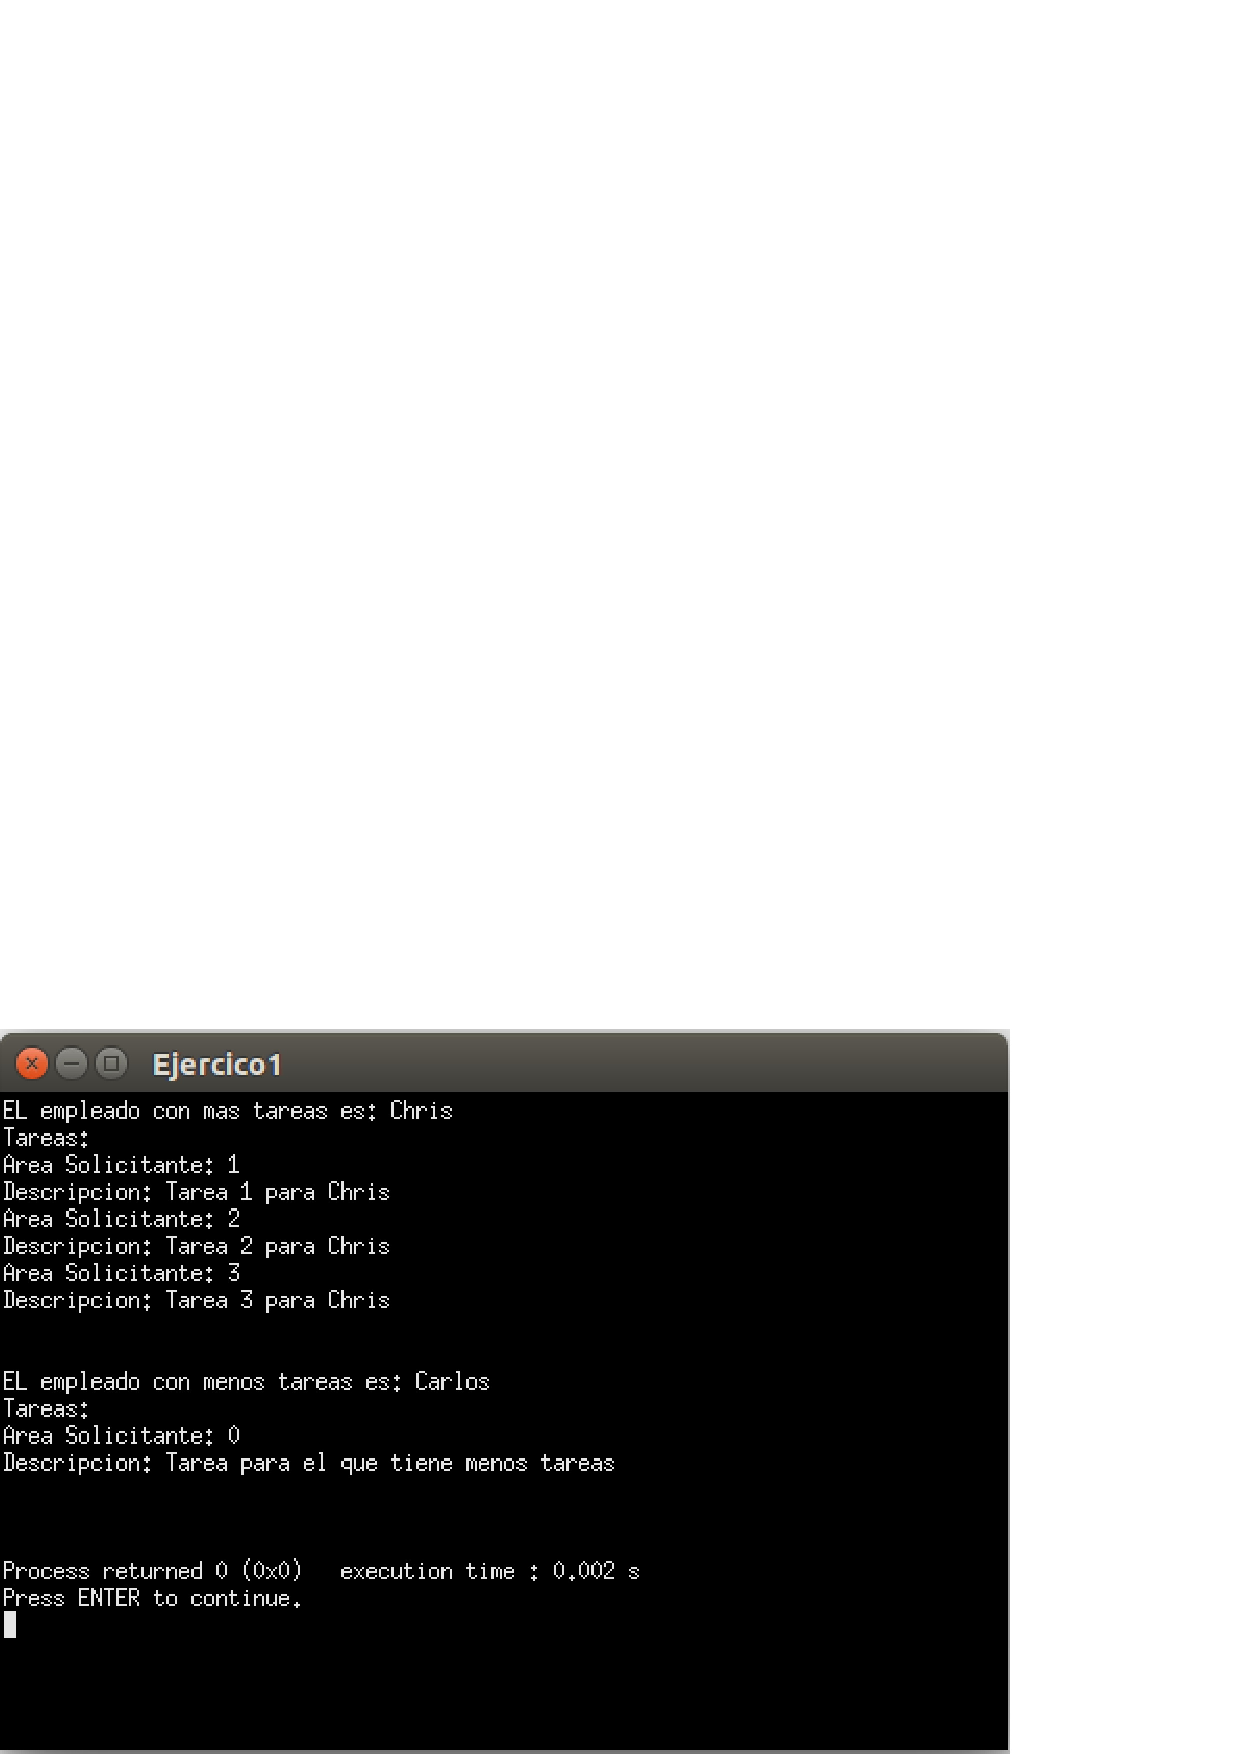
\includegraphics[scale = 0.5]{1.png}
 \end{figure}
 \item $n=25$
 \begin{figure}[h]
  \centering
  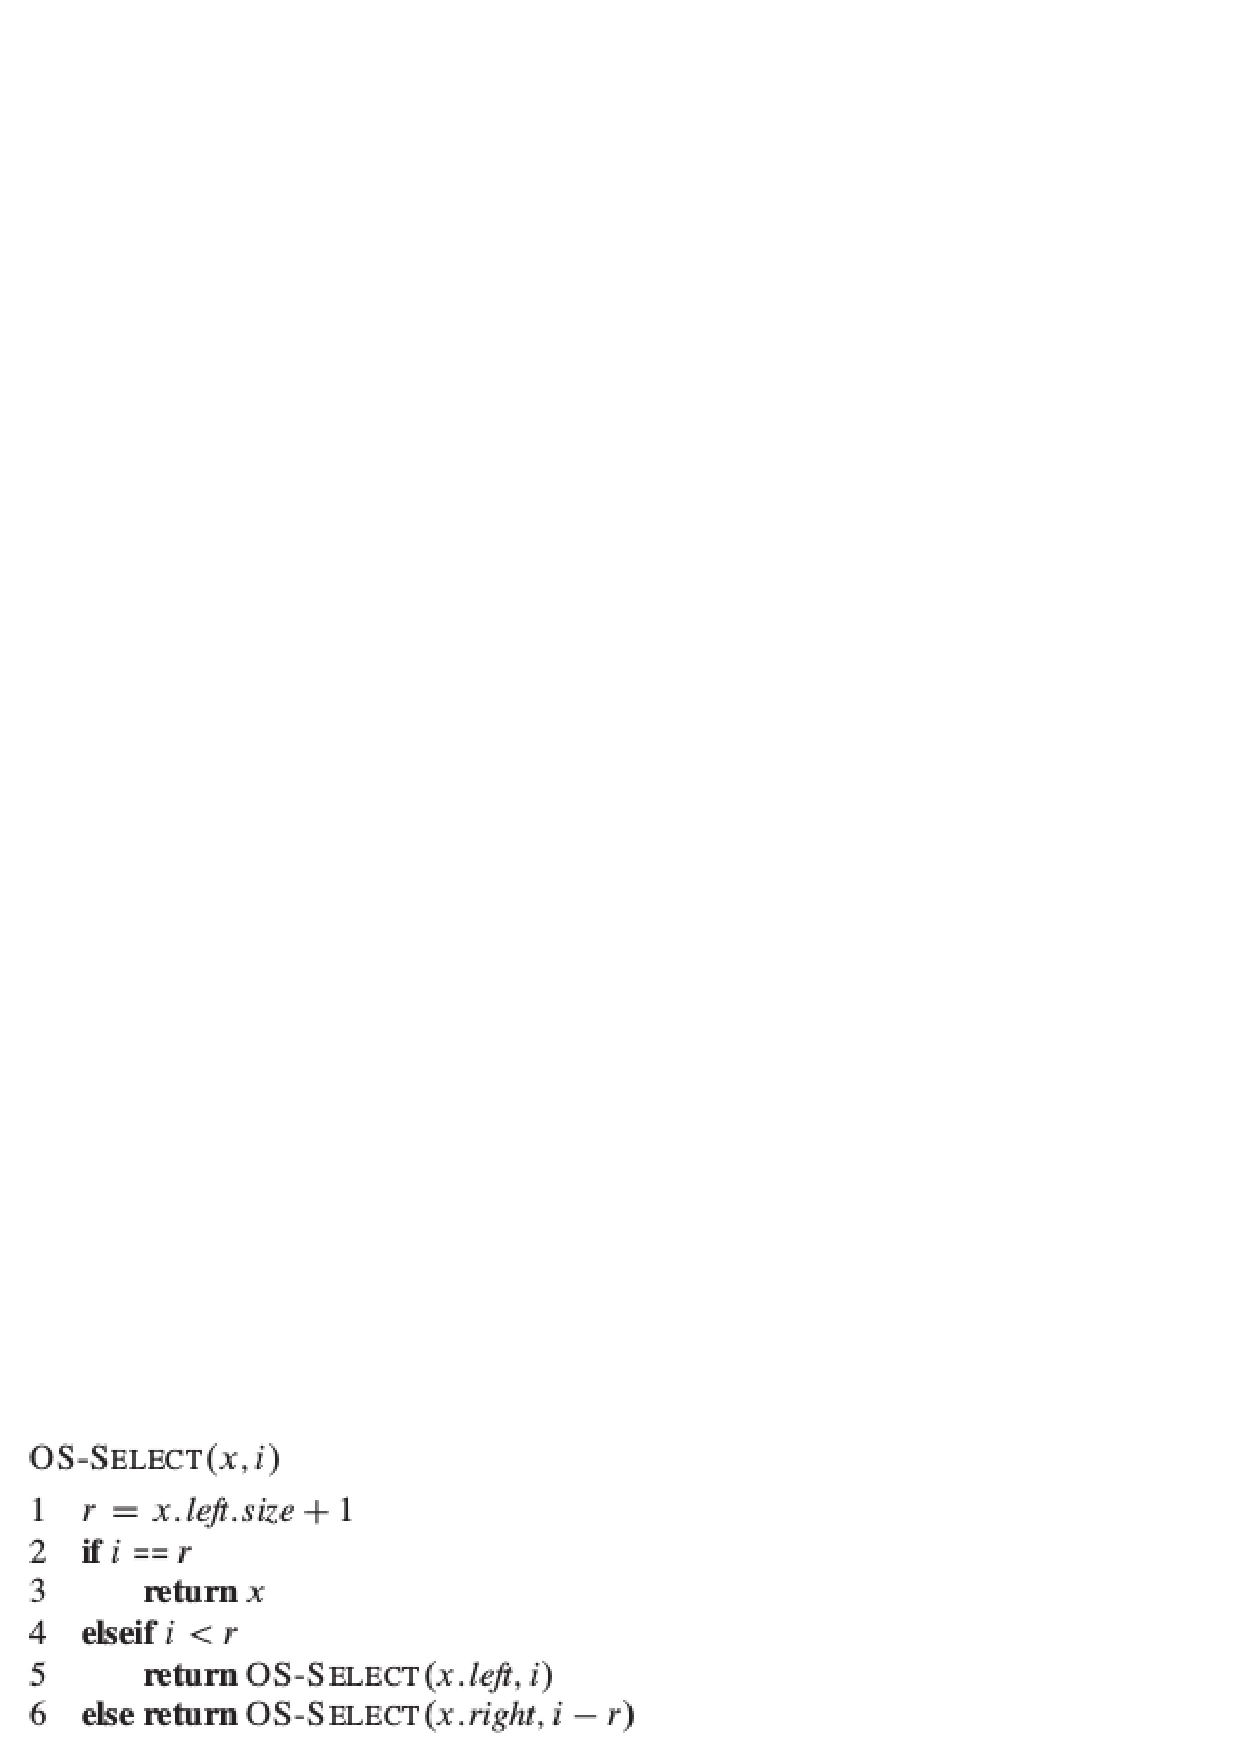
\includegraphics[scale = 0.5]{2.png}
 \end{figure}
  \item $n=100$
  \begin{figure}[h]
   \centering
   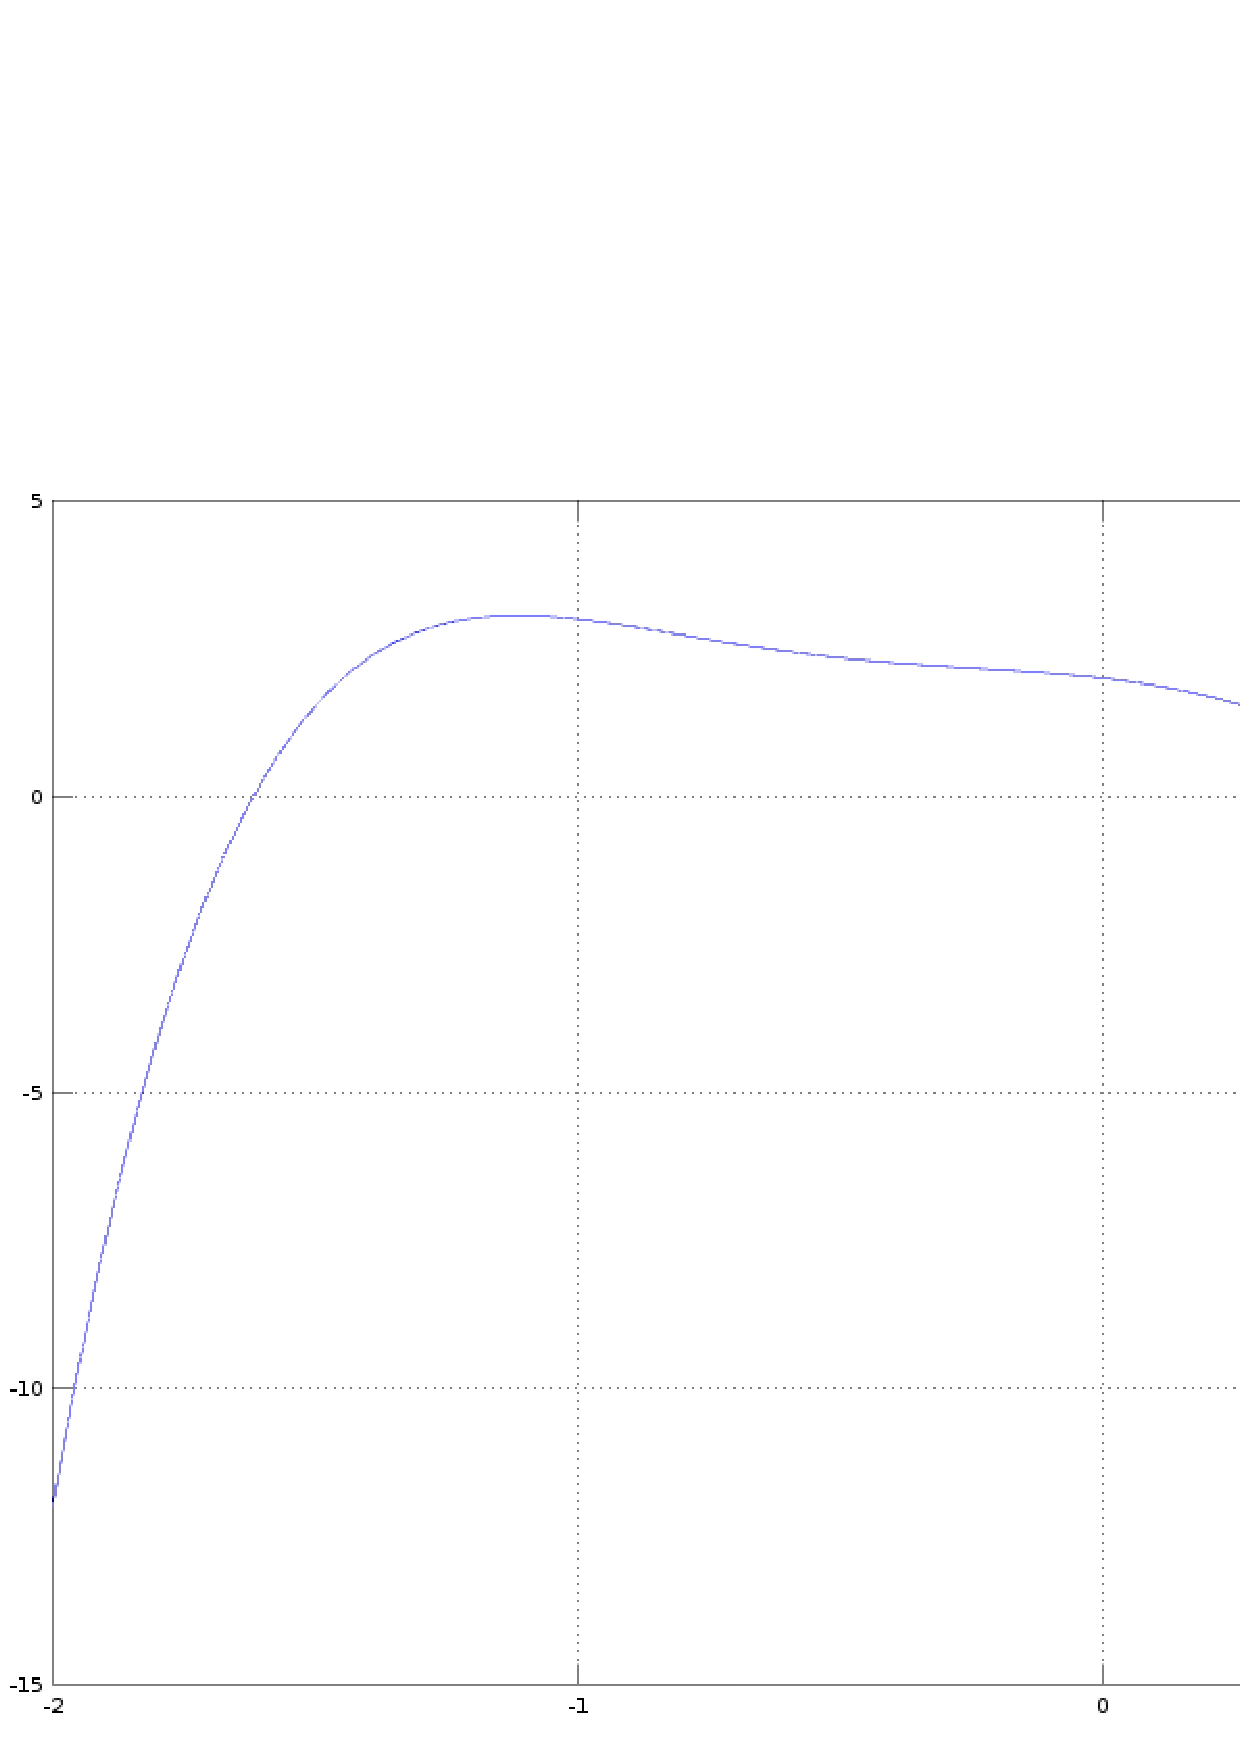
\includegraphics[scale = 0.5]{3.png}
  \end{figure}

\end{itemize}


\end{document}
